\documentclass[11pt,a4paper]{article}
\usepackage[utf8]{inputenc}
\usepackage{a4wide}
\usepackage{fancyhdr}
\pagestyle{fancy}
\thispagestyle{fancy}

\usepackage{gensymb}
\usepackage{hyperref}
\newcommand\fnurl[2]{%
  \href{#2}{#1}\footnote{\url{#2}}%
}
\usepackage{amsfonts}
\usepackage{natbib}

\usepackage[spanish]{babel}
\parskip = 11pt

\usepackage{tabularx}

\usepackage[conEntregas]{caratula}
\materia{Ingenier\'ia del Software 2}
\titulo{Trabajo Pr\'actico I}
\subtitulo{\textit{Curry Game}}
\integrante{Aleman, Dami\'an Eliel}{}{damianealeman@gmail.com}
\integrante{Arjovsky, Mart\'in}{}{martinarjovsky@gmail.com}
\integrante{Fixman, Mart\'in}{}{martinfixman@gmail.com}
\integrante{Harari, Ignacio}{}{nachotee@hotmail.com}

\def\tabularxcolumn#1{m{#1}}

\begin{document}

\maketitle

\section*{User Stories}

Las User Stories mostradas en \textbf{negrita} son las ser\'an completadas en el primer Sprint.

\begin{table}[h]
\begin{tabularx}{\textwidth}{|X|c|c|}
\hline
\textbf{Descripci\'on} & \textbf{Esfuerzo} & \textbf{  Value  } \\ \hline
Como participante quiero poder registrar una cuenta para acceder al juego. & \Large2 & \Large8  \\ \hline
Como participante quiero buscar desafíos para poder aceptarlos. & \Large5 & \Large5 \\ \hline
Como participante quiero armar equipos para poder aceptar o postular desafíos con ese equipo. & \Large3 & \Large5 \\ \hline
Como administrador quiero administrar jugadores disponibles para poder organizar el juego. & \Large3 & \Large2 \\ \hline
Como administrador quiero consultar las cuentas que están en el sistema para poder analizar el uso del juego por los participantes. & \Large5 & \Large2\\ \hline
Como participante quiero autenticar mi cuenta (log in) para poder entrar en el sistema de juego. & \Large2 &\Large8 \\ \hline
Como participante quiero poder ver mi cap y mis fichas para decidir mis apuestas. &\Large2 &\Large3 \\ \hline
Como participante quiero ver tabla de posiciones de todos los participantes en base a sus desafíos ganados/perdidos para poder conocer el ranking. & \Large3 & \Large2\\ \hline
Como participante quiero postular desafío para desafiar a otros participantes a que jueguen contra mi equipo. & \Large2 & \Large5 \\ \hline
Como participante quiero aceptar el desafío postulado por otro participante para poder jugar contra otros equipos. & \Large2 & \Large5 \\ \hline
Como administrador quiero poder crear jugadas ofensivas y defensivas. &\Large5&\Large3 \\ \hline

\textbf{Como administrador quiero poder simular una acción ofensiva y defensiva.} &\Large5 & \Large8 \\ \hline
\textbf{Como administrador quiero editar fórmulas y números  de resolución de acciones para poder cambiar el juego en caso de que se necesite.} & \Large5 & \Large3\\ \hline
\textbf{Como participante quiero ver log del partido e información pertinente para poder visualizar las simulaciones anteriores.} & \Large3 &\Large8 \\ \hline
\textbf{Como participante quiero nombrar mi equipo, elegir mi jugador estrella y mi tecnico.} & \Large2&\Large5 \\ \hline
\end{tabularx}
\end{table}

\begin{itemize}
	\item La \textbf{P\'agina Web} le pide al controlador de partidos la simulaci�n v�a un client server. Controlador de partido realiza la simulaci�n pidiendo la data necesaria al calculador de puntos. Luego escribe el resultado en el log minuto a minuto y le manda los pedidos de video al controlador de engine. Este �ltimo decide si hacer video 2d o 3d y pide el video al engine correspondiente. Acto seguido, controlador de engine pone el video simulado en un pipe al controlador de partidos para que se los mande a la p�gina web.
	\item El \textbf{Sistema de Pagos y Cobros} se ocupa de la comunicaci\'on del sistema con el banco y con la tarjeta de cr\'edito para cobrarle dinero al usuario (y obtener cr\'editos) o devolverle dinero que puede haber comprado o ganado en apuestas (y, asumiendo que tenga los cr\'editos suficientes, cobrarselos).
	\item El \textbf{Calculador de Puntos} calcula los puntos correspondientes a una jugada con informaci\'on obtenida del Control de Partido. Este usa f\'ormulas sacadas de la base de datos, y le pide datos de los jugadores en las redes sociales al \textit{Calculador de Puntos de Popularidad}.
	\item El \textbf{Controlador de Popularidad} tiene la responsabilidad de buscar en las redes sociales informaci\'on sobre qu\'e est\'a diciendo la gente sobre cada jugador, as\'\i se puede saber cu\'antos puntos se deben agregar. Esta informaci\'on es recolectada por el \textit{Scraper}, que consigue datos de \textit{Facebook} y \textit{Twitter}, y enviada al \textit{Int\'erprete de Texto}, que devuelve una serie de ``keywords'' al Controlador.
	\item El \textbf{Controlador de Engine} es activado por el \textit{Controlador de Partido}, que tambi\'en le env\'{\i}a las propiedad del sistema para saber si debe usar el \textit{Engine 3D} \'o el \textit{Engine 2D}. Dependiendo de la informaci\'on prove\'{\i}da por este y lee el \textit{Log Minuto a Minuto} para crear la simulaci\'on gr\'afica del partido, que env\'{\i}a de vuelta al control del partido.
	\item El \textbf{Apostador} recibe datos de apuestas de un usuario desde la p\'agina web y de sus cr\'editos. Luego de terminado un partido, este cobra o agrega cr\'editos al usuario.
	\item El \textbf{Administrador de Desaf\'{\i}os} administra los partidos que todav\'{\i}a no fueron concretados, y que los usuarios pueden aceptar o no. El \textit{Administrador Web} le comunica que hay un nuevo desaf\'{\i}o o que uno ya existente fue aceptado, y en el \'ultimo caso lo guarda en la base de datos de desaf\'{\i}os y activa la cuenta regresiva. Cuando este termina, le env\'{\i}a al \textit{Controlador de Desaf\'{\i}os} que el partido debe comenzar, y este le adelanta la notificaci\'on al \textit{Controlador de Partido}.
\end{itemize}


\section{Seguimiento}

Aquí explicaremos algunas de las problemáticas que nos fuimos encontrando al resolver el trabajo, las alternativas que nos planteamos, las soluciones en las que concluímos y las razones de éstas decisiones.

\subsection{Contraataque}

Representar al contraataque dentro de la aplicación, por tener características especiales que no comparte con el resto de las estrategias ofensivas, fue desde un principio un problema. Antes de llegar a la solución final que elegimos, ya explicada anteriormente, discutimos otras que terminamos descartando por diversos motivos. Por ejemplo, una de las alternativas incluía mantener al contraataque como una \textbf{EstrategiaOfensiva}, y crear entonces dos \textbf{Acciones Ofensivas} nuevas que representaran un \textbf{Tiro Inbloqueable} (de 2 y 3 puntos). 

Los problemas de tener esas acciones, y de modelar al contraataque como una estrategia ofensiva (en el contexto de nuestro modelo) eran varios, en principio, el contraataque como estrategia debía exluirse de poder ser elegido por un tícnico como estrategia ofensiva, y de modelarlo con Tiros Inbloqueables, habría requerido una seccion especial en el método de \textbf{simular} que chequeara luego de cada intercepción si debíamos inicializar un contra ataque o no, y tendríamos que haber decidido la manera de elegir si debíamos hacerlo o no, que no nos era del todo clara ya que no estaba especificada. En pos de mantener al método de \textbf{simular} lo más genérico posible y agnóstico el tipo de Jugada que se esté simulando, decidimos cambiar un poco la interpretación de la manera que ya fue explicada, y encapsular el comportamiento especial en su propio método del simulador.

Una solución alternativa que no implementamos por su complejidad, pero que podría haber sido más genérica (y entonces, más modificable) de haberla pensado hasta el final era la de tener una serie de \textbf{ModificadoresDeExito} que pudieran agregarse a las \textbf{Acciones}, y que serían llamados para modificar la probabilidad de éxito desde la \textbf{Acción} (en el momento en el que ésta calcula su triunfo), junto con una suerte de \textbf{Tabla de Efectividad}, que sería un objeto encargado de saber la efectividad de una estretegia ofensiva particular contra otra estrategia defensiva, y viceversa, devolviendo los \textbf{Modificadores} correspondientes. Esto nos habría permitido modelar el contraataque agregando a la Tabla la regla de que, cuando se realiza un contraataque, las acciones defensivas deben llevar un modificador que las hace inefectivas (ya que así está definido en el enunciado), y nos habría permitido definir otros modificadores de la aplicación, como es el cansancio que resulta de ejecutar una jugada MvP de manera similar.

\subsection{Simulación}

La simulación del partido es claramente la parte más complicada de la aplicación, desde el punto de vista de diseño, por lo que tuvimos que iterar sobre muchas soluciones fallidas hasta llegar a algo satisfactorio, la clave aquí fue el Double Dispatch. El inconveniente se encontraba en, dada una estrategia ofensiva, y una defensiva, necesitabamos saber exáctamente con qué \textbf{Accion Defensiva} responder a la \textbf{Acción Ofensiva} que estuvieramos analizando en ese momento; dentro de las opciones posibles barajamos la idea de tener una suerte de Map que funcionara como oráculo al cual, al darle las estrategias, nos devolviera los objetos correctos para continuar la simulación, pero si bien eso encapsularía la decisión, requeriría tener \textbf{if's} dentro de ella de alguna manera, con lo cual al llegar a la solución de Double Dispatch concluimos entre todos que era un mucho mejor diseño.


\section{Retrospectiva General}
En líneas generales después de realizar el product backlog se nos hizo muy difícil
realizar las tareas a tiempo como estaba estipulado para lograr un burndownchart
con una velocidad relativamente constante, que sería lo ideal. 
Sin embargo creemos que esto no es debido a la metodología de trabajo ya que 
ésta realiza retrospectivas de forma constante justamente para que 
no ocurran estas problemáticas de tiempos.
Al ser un trabajo práctico, es decir un trabajo que no se realiza a diario 
es más difícil tener la constancia necesaria
para realizar adecuadamente estos tipos de metodologías ágiles.


\section{Escenarios}

\subsection{Crear Equipo}

En el siguiente escenario unParticipante crea un equipo eligiendo con el nombre Pipe\&Filter, el tecnico Popovich, el base LeBron James,escolta Kevin Durant, alero ShaquilleONeal, ala pivot Michael Jordan y como pivot Kobe Briant. 

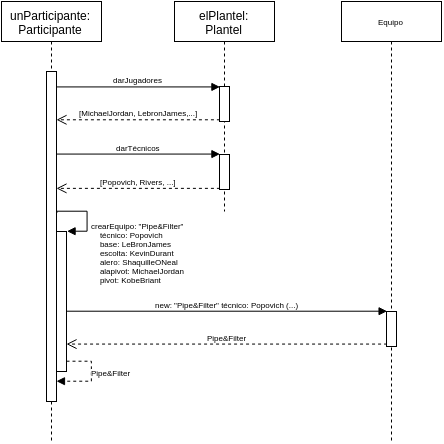
\includegraphics[width=\textwidth]{imgs/crearEquipoSecuencia.png}

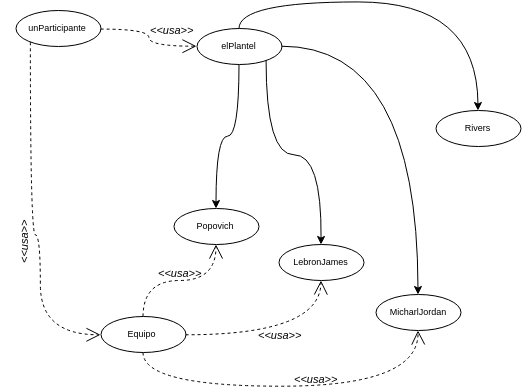
\includegraphics[width=\textwidth]{imgs/crearEquipoObjetos.png}



\subsection{Aceptar Desafío}
En este escenario otroParticipante elige de un pool de Desafíos el desafío donde está el equipo Pipe\&Filter apostando 5 fichas y lo acepta con su equipo llamado Batch. Luego el partido se simula y gana el equipo Pipe\&Filter 97 a 92 generando una ganancia de 15 fichas para unParticipante y una perdida de 5 fichas para otroParticipante. 

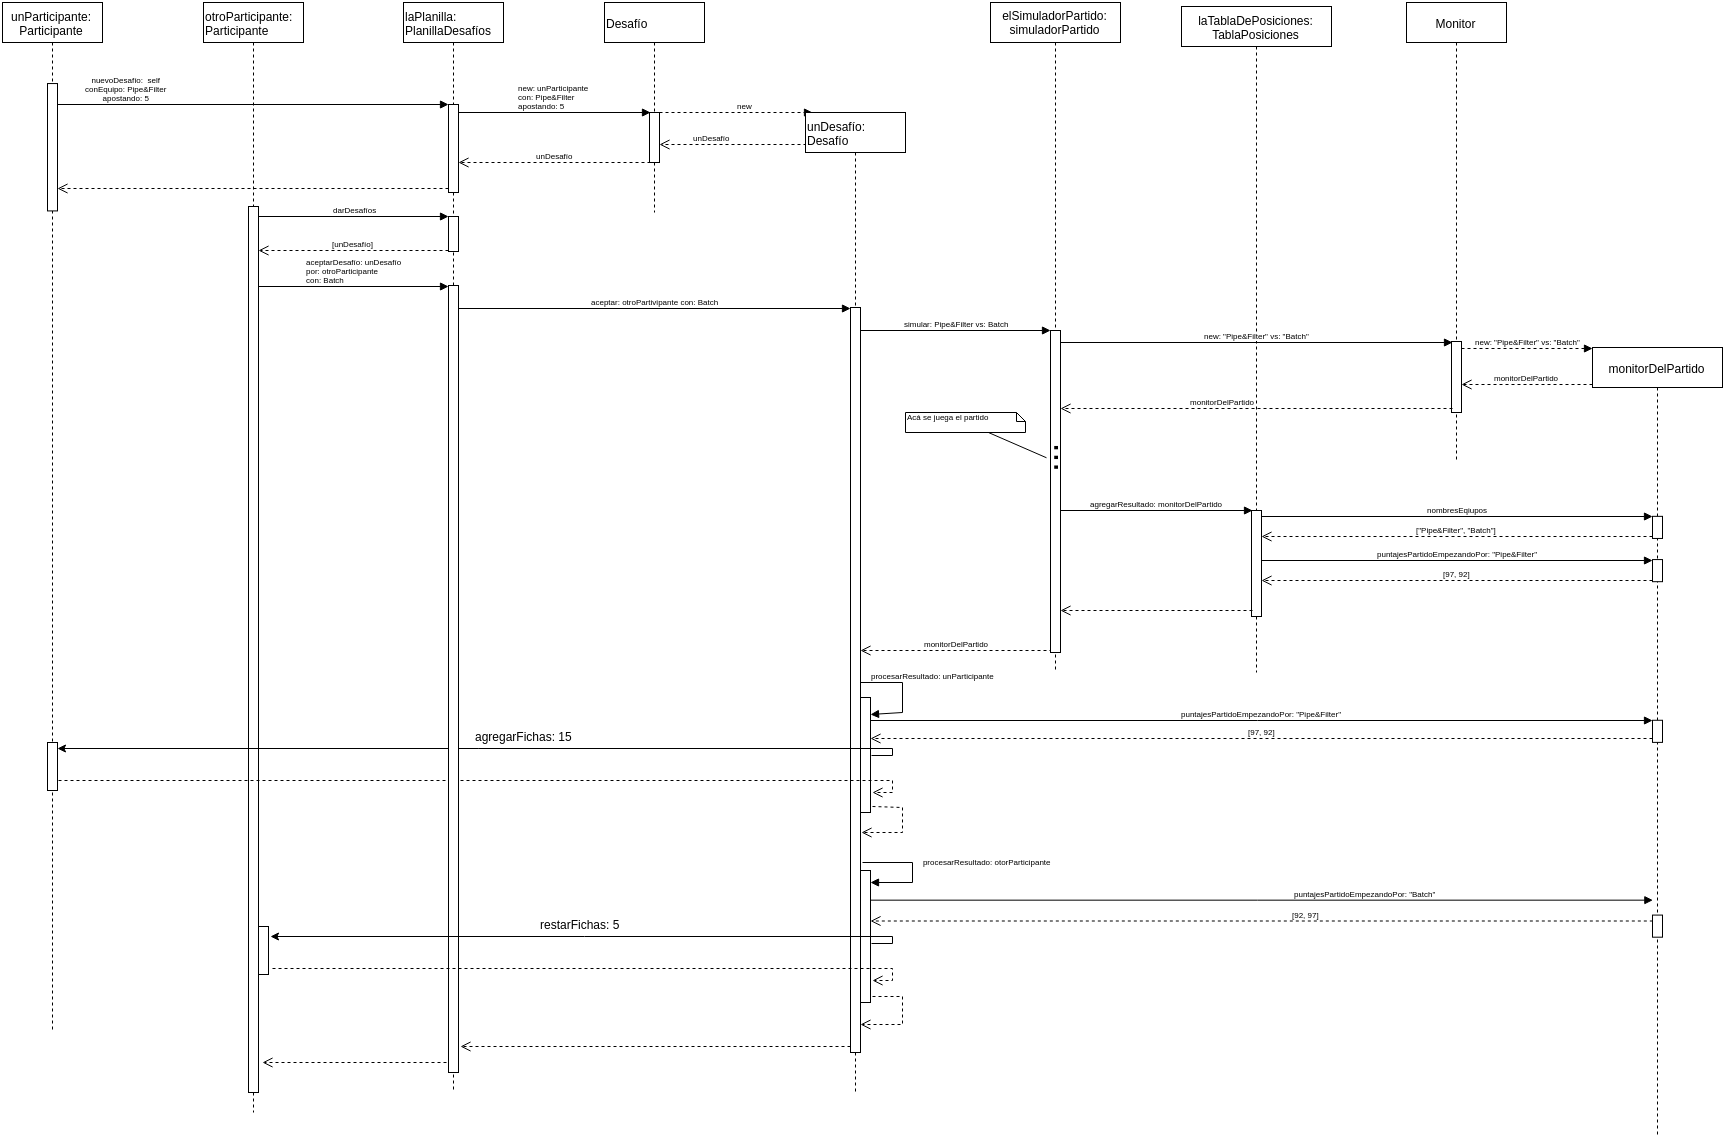
\includegraphics[height=0.7\textheight,keepaspectratio, angle =90 ]{imgs/aceptarDesafioSecuencia.png}

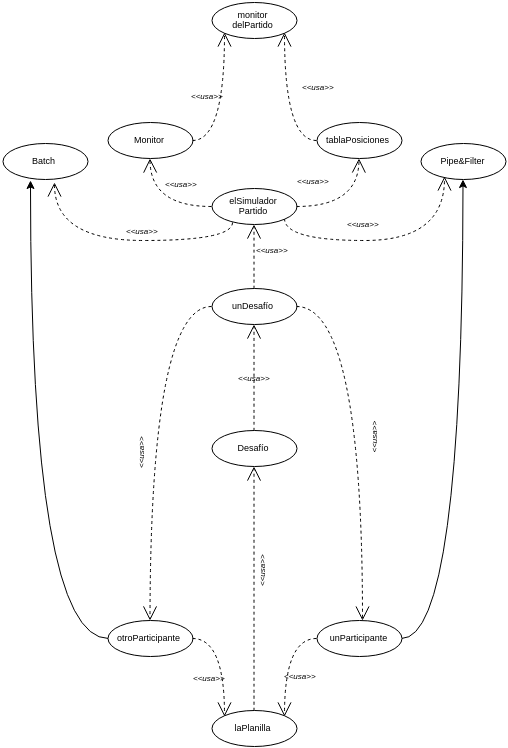
\includegraphics[width=\textwidth]{imgs/aceptarDesafioObjetos.png}

\subsection{Pase Exitoso}

El siguiente diagrama muestra una secuencia de mensajes de un pase que es exitoso. Esta secuencia estará en las simulaciones del simuladorDeTurno.

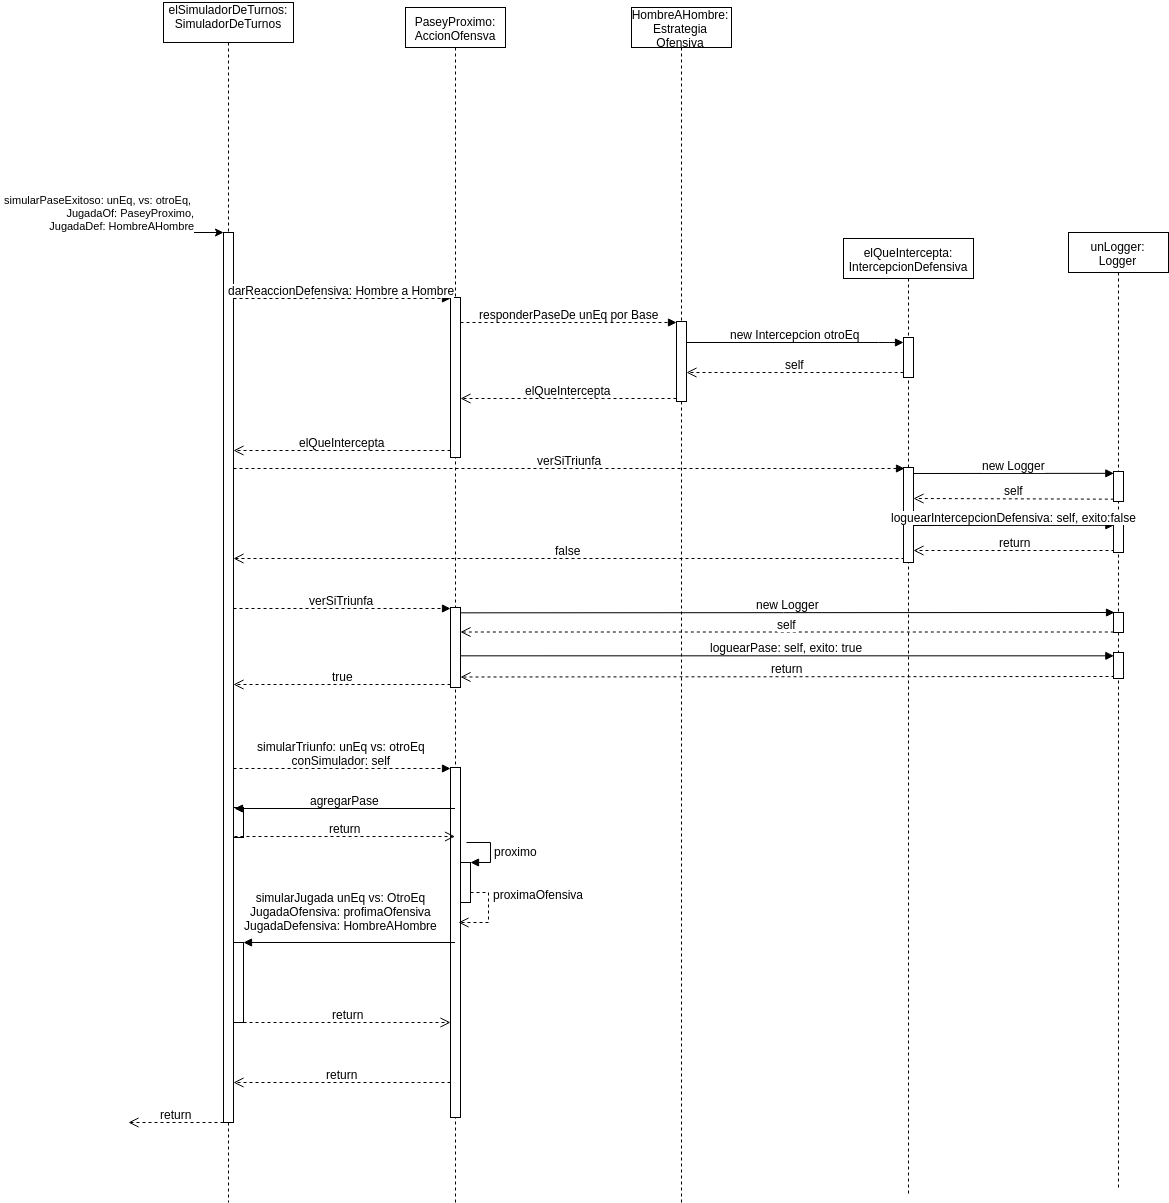
\includegraphics[width=\textwidth]{imgs/PaseExitoso.png}

\subsection{Pase Fallido}

Análogamente para el Pase Fallido

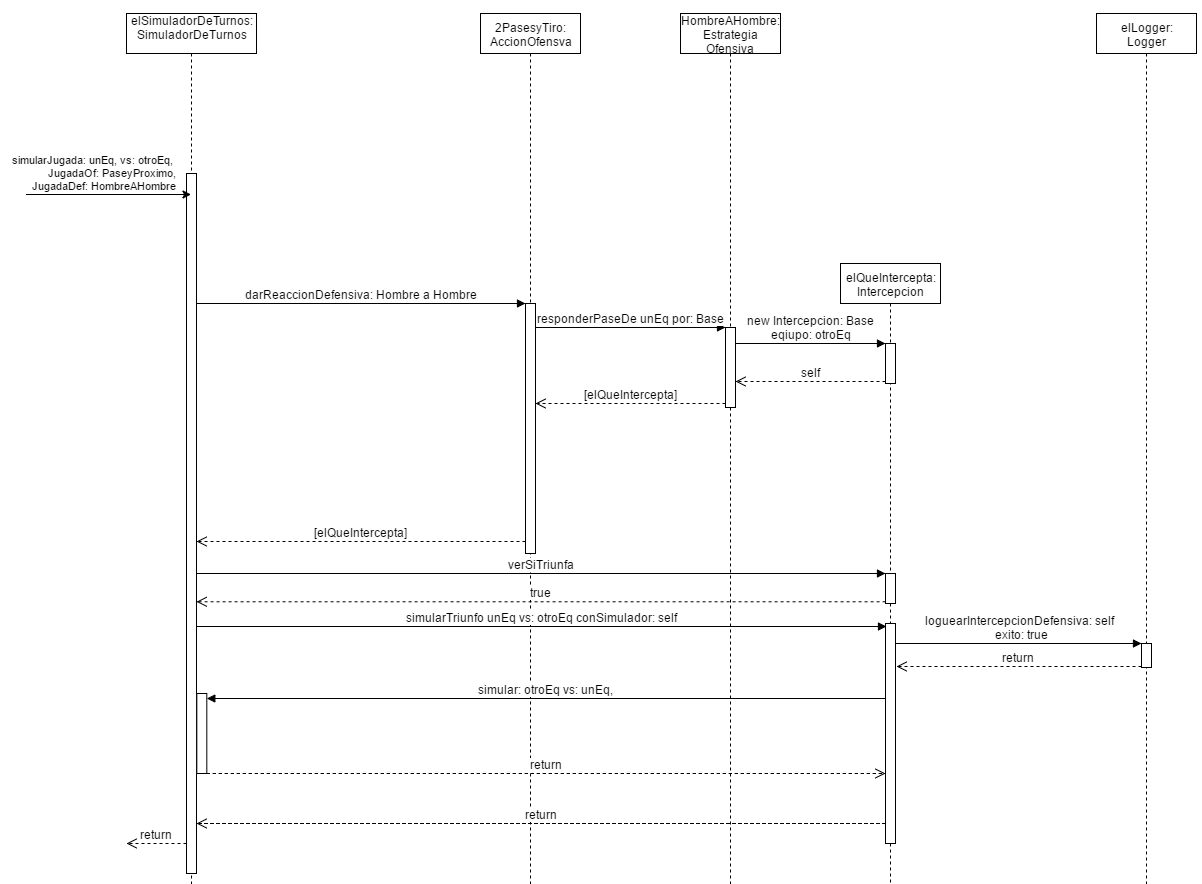
\includegraphics[width=\textwidth]{imgs/PaseFallido.png}

\subsection{Tiro Exitoso}

El siguiente diagrama muestra una secuencia de mensajes de un tiro que es exitoso. Esta secuencia estará en las simulaciones del simuladorDeTurno.

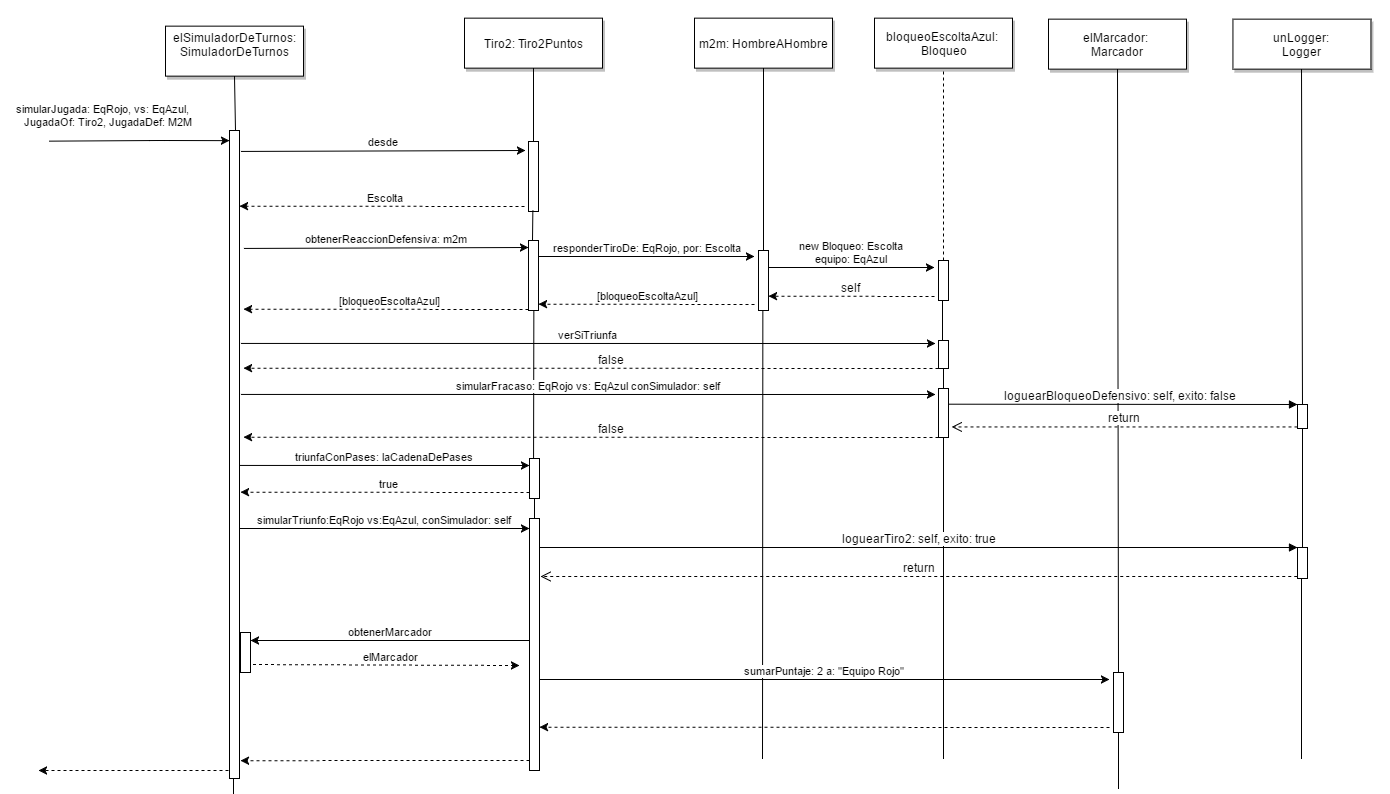
\includegraphics[width=\textwidth]{imgs/TiroExitoso.png}

\subsection{Tiro Fallido}

Análogamente para el Tiro Fallido

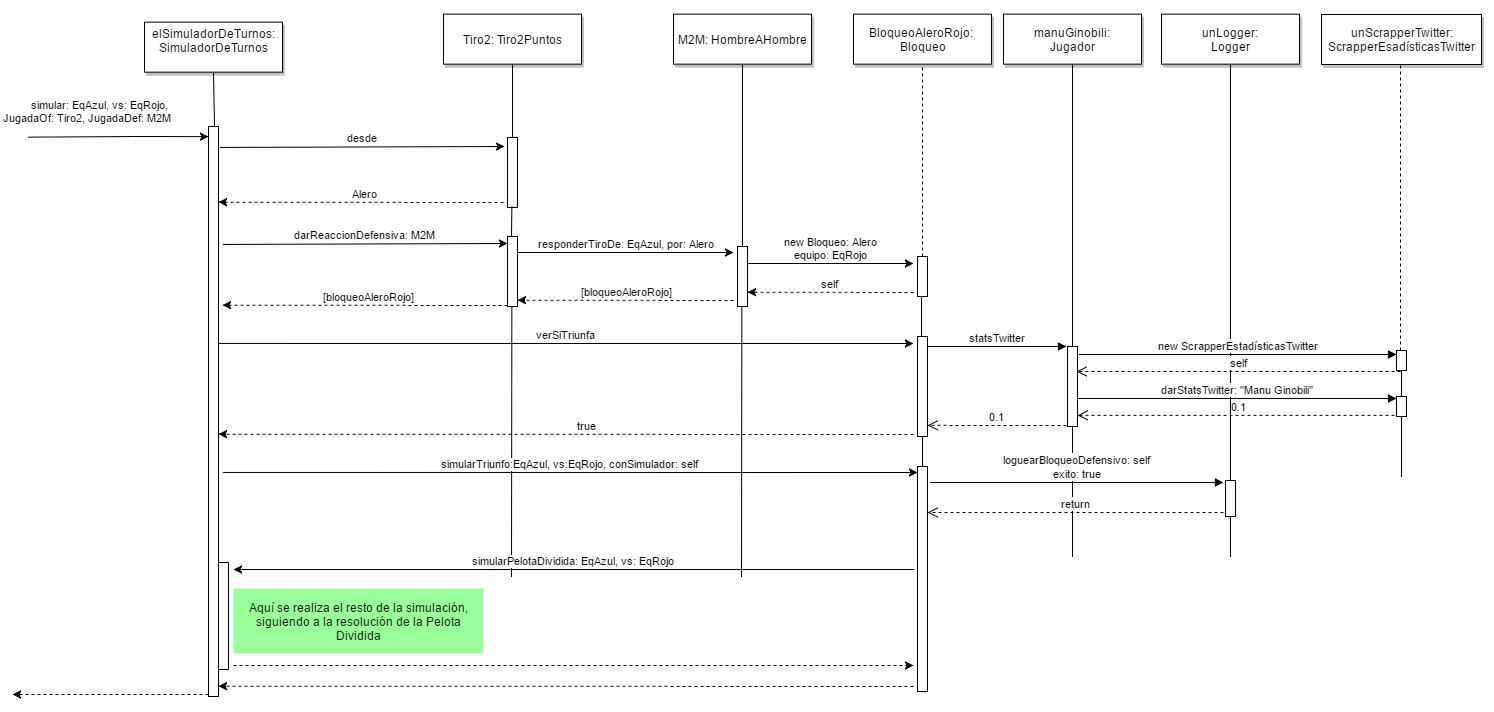
\includegraphics[width=\textwidth]{imgs/TiroFallido.png}

\subsection{Pelota Dividida}
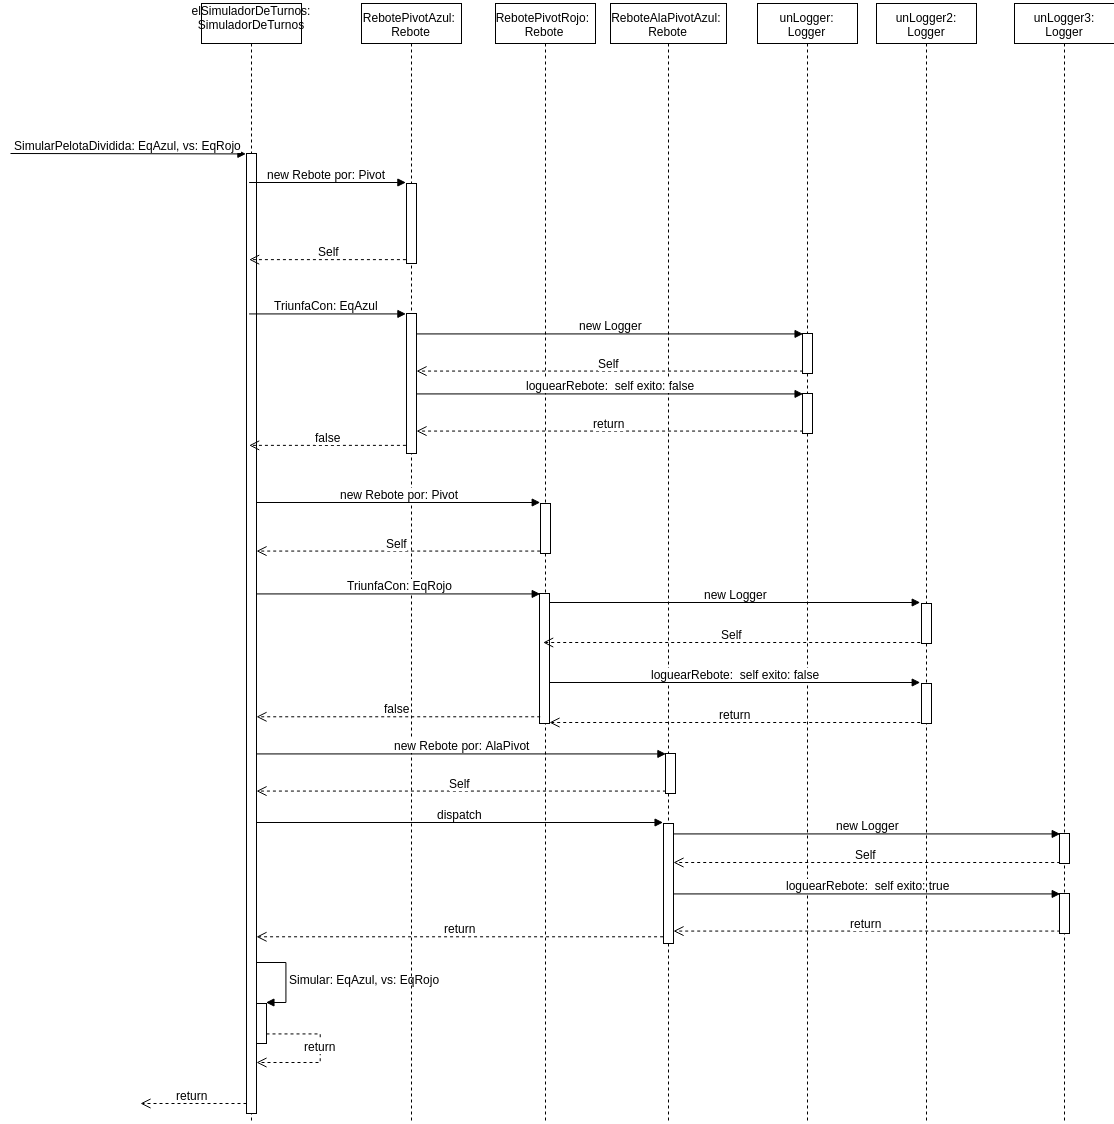
\includegraphics[width=\textwidth]{imgs/PelotaDivididaSecuencia.png}

\subsection{Colectiva Externa de 3}

El siguiente diagrama muestra un escenario donde en una jugada el equipo atacante (unEq) hace dos pases y un tiro y encesta, teneiendo como estrategia Colectiva Externa de k pases.

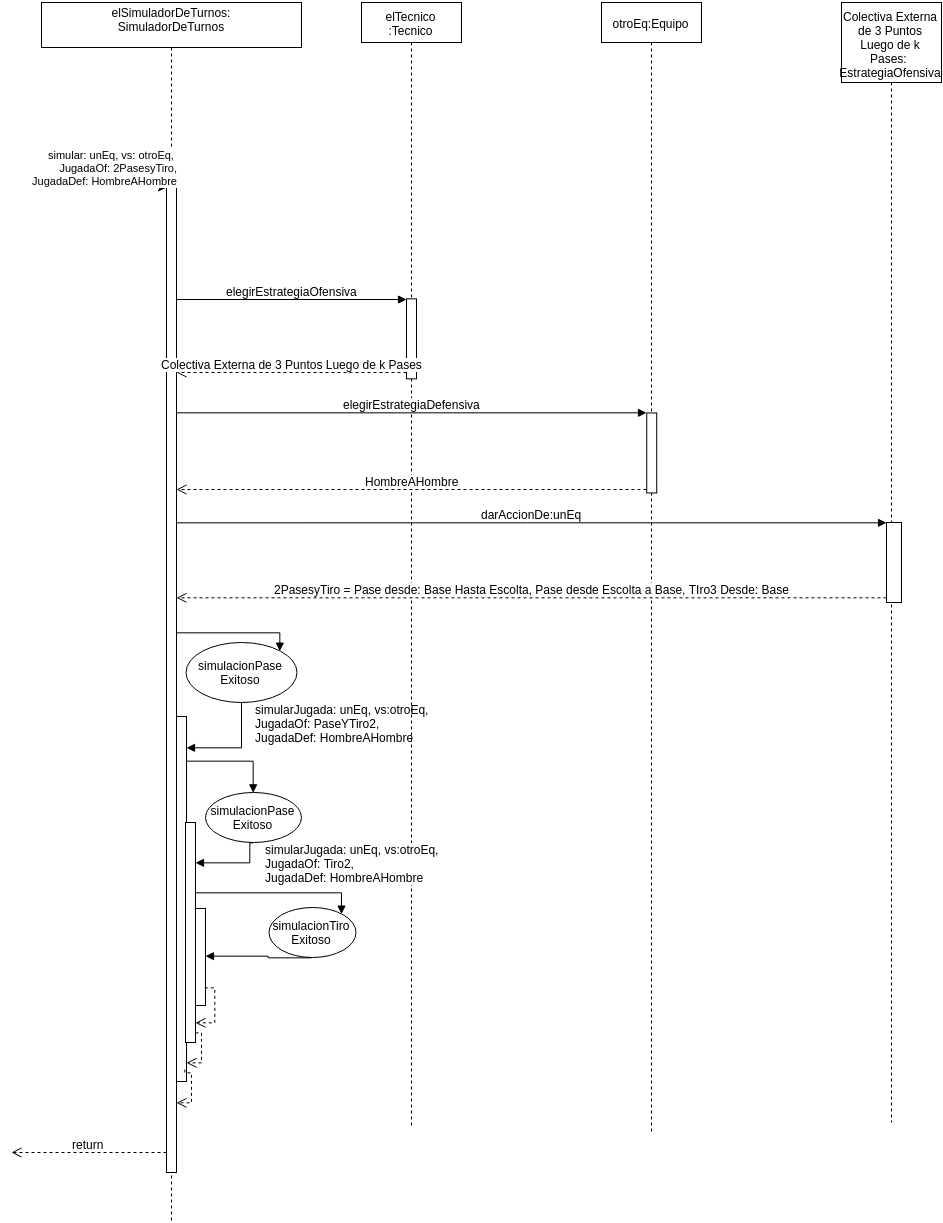
\includegraphics[width=\textwidth]{imgs/colectivaExternaDe3Secuencia.png}

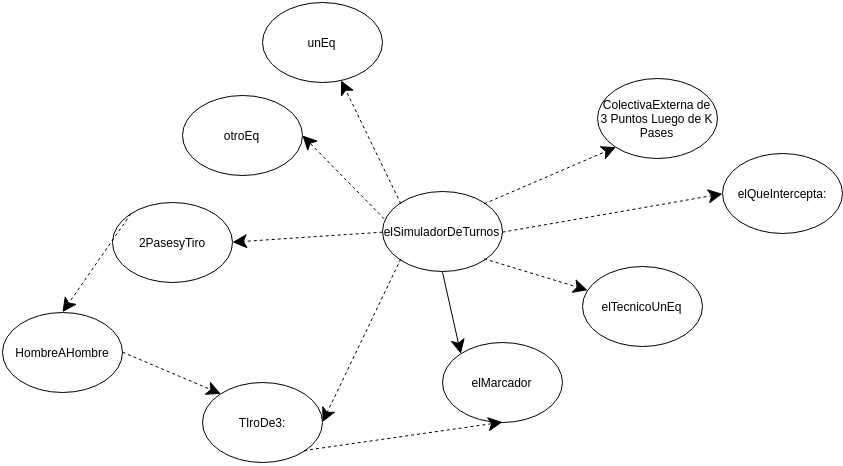
\includegraphics[width=\textwidth]{imgs/colectivaExternaDe3Objetos.png}

\subsection{Contraataque}
El siguiente diagrama muestra un escenario donde en una jugada el equipo atacante (eqAzul) hace un pase do forma exitosa, en el segundo pase es interceptado por el otro equipo y este ultimo tira al aro encestando sumando 2 puntos al marcador para su equipo.
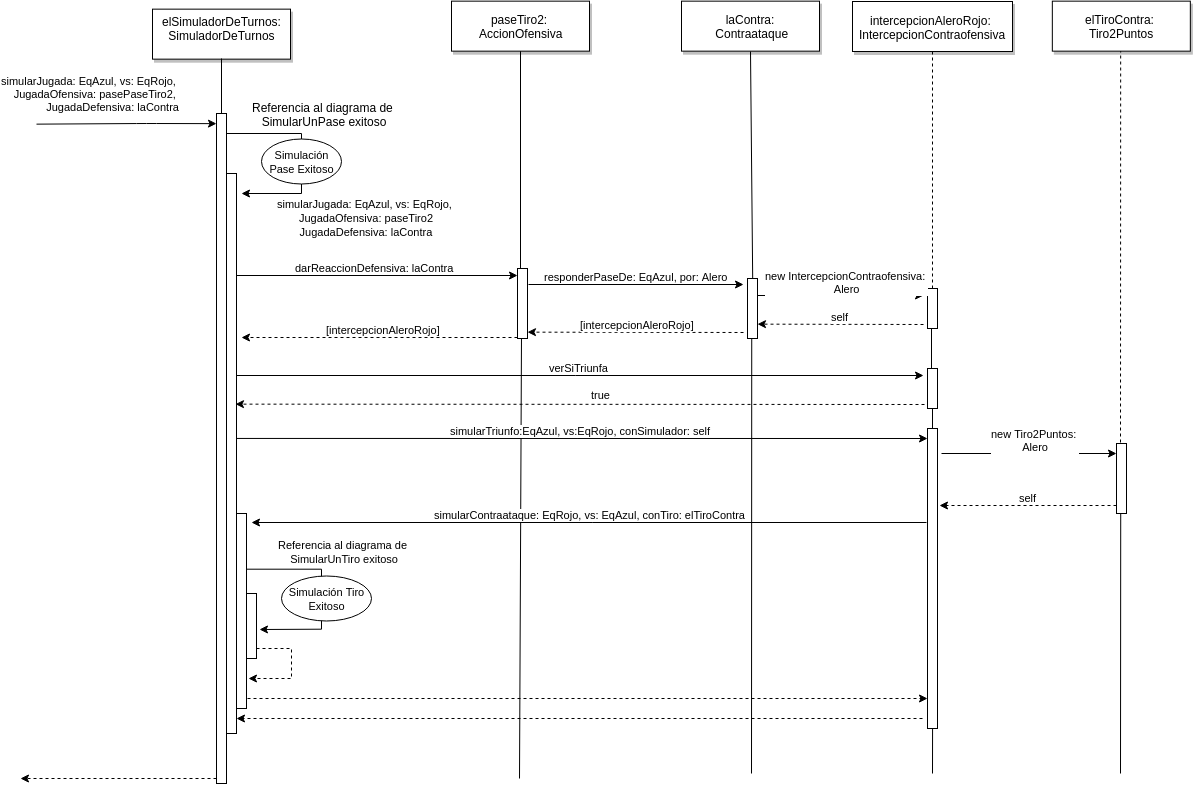
\includegraphics[width=\textwidth]{imgs/ContraataqueSecuencia.png}




\end{document}
